
\documentclass[12pt]{article}
\pagestyle{empty}
\setlength{\parskip}{0in}
\setlength{\textwidth}{6.8in}
\setlength{\topmargin}{-.5in}
\setlength{\textheight}{9.3in}
\setlength{\parindent}{0in}
\setlength{\oddsidemargin}{-.7cm}
\setlength{\evensidemargin}{-.7cm}

\usepackage{amsmath}
\usepackage{amsthm}
\usepackage{amstext}

\usepackage{graphicx}

\begin{document}


\textbf{MAT 105 Exam 1 (ivory) Summer 2010} \hspace{.4in} {\large Name} \hrulefill

\begin{center}

\begin{tabular}
{|l|c|c|c|c|c|c|c|c|c|c|c|c|c|} \hline

 Problems & \hspace{5 pt} 1 \hspace{5 pt}  & \hspace{5 pt} 2 \hspace{5 pt} & \hspace{5 pt} 3 \hspace{5 pt} & \hspace{5 pt} 4 \hspace{5 pt} & \hspace{5 pt} 5 \hspace{5 pt} & \hspace{5 pt} Total  \hspace{5 pt} & &  \hspace{5 pt} Grade \hspace{5 pt}  \\ \hline
&&&&&&&&\\  
Points &&&&&&&    \hspace{.8in}\% &  \\ 
&&&&&&&& \\  \hline
Out of & 12 & 32 & 32 & 14 & 10 &100 & & \\ \hline

\end {tabular}

\end{center}

\vspace{.2in}

 \emph{Relax.  You have done problems like these before.  Even if these problems look a bit different, just do what you can.  If you're not sure of something, please ask! You may use your calculator.  Please show all of your work and write down as many steps as you can.  Don't spend too much time on any one problem.  Always remember to report the units on an answer. Do well.  And remember, ask me if you're not sure about something.} \\

\vspace{.5in} 
\noindent \emph{A few formulas from our book:}
\begin{center}

\textbf{Root Formula:} 

A solution of the equation $B^n=k$ is $B=k^{1/n}$.

\vspace{.2in} 

\textbf{Percent Increase Formula:} 

To get the result of increasing an amount by $r$\%, multiply by $1 + \frac{r}{100}$.

\end{center}

\hrulefill

%%%%%%%%%%%

\newpage

%%% Old 1.3, public health, citizen
\begin{enumerate}
\item The graph below shows the total number of people who contracted the flu last year ($I$, in thousands of people) $D$ days after November 1.  Use the graph to answer the following questions.

\begin{center}
\scalebox {.7} {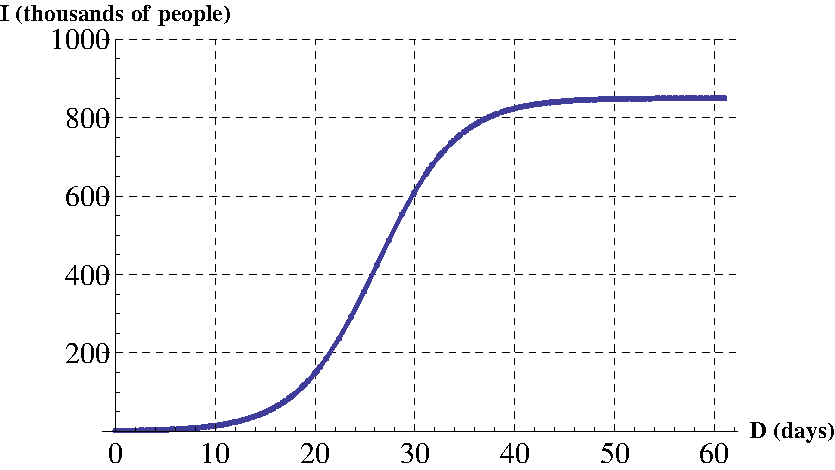
\includegraphics [width = 8in] {flu}}
\end{center}



\begin{enumerate}
\item Approximately how many people had the flu 20 days after November 1? 
\vfill
\item Does this graph show a dependency that is increasing, decreasing, or neither?
\vfill
\item Approximately what day did the number of people with the flu exceed 700,000 (=700 thousand) people?
\vfill
\item This graph only shows data to the end of the year (December 31).  If the graph continued into the new year, what do you think it would look like?  Describe your reasoning with a sentence or two.
\vfill
\end{enumerate}
\newpage
%%%%%%%%%%%%%%%%%%%%%%%%%
%%% Old 1.6, home, everyday
\item  To hire an handyman to fix my broken garage door it costs \$95 for the service call plus a \$50 hourly rate.

\begin{enumerate}
\item Make a table showing the cost of the handyman's visit if he works for 1 hour, 3 hours, and 7 hours. 
\vfill
\item Name the variables, including units, and write an equation illustrating the dependence.
\vfill
\item The bill for the handyman's work was \$345.  Solve your equation to determine how long he worked.  \emph{If you cannot solve the equation, you may show some other method of finding the answer for possible partial credit.}
\vfill
\item Draw a graph showing how the handyman's bill changes with his hours worked.
\vspace{.1in}
\begin{center}
\scalebox {.8} {
\includegraphics [width = 6in] {../GraphPaper}}
\end{center}
\vspace{.1in}
\end{enumerate}
%%%%%%%%%%%%%%%%%%%%%%%%%%%%%%%%%%%
\newpage

%%% Old 1.8, population, citizen?
\item The CIA world factbook estimated that the population of Costa Rica is growing at a rate of 1.3\% per year.  In 2008 the population was estimated to be 4.2 million.  

\begin{enumerate}
\item Write an equation illustrating this dependence using the following variables:

\quad $P= $ population (measured in millions of people)

\quad $Y = $ year (measured in years since 2008)

\vfill
\item Make a table showing the population in 2008, 2013, 2018, and 2023. Please report your answer to the first decimal place.
\vfill
\item Draw a graph showing how population will change in the future.
\vspace{.1in}
\begin{center}
\scalebox {.8} {
\includegraphics [width = 6in] {../GraphPaper}}
\end{center}
\vspace{.1in}
\item Use successive approximations to predict when the population will rise above 5 million.  Please report your answer to the first decimal place.   \emph{Display your work in a table.  Answer to the nearest year.  Be sure to say the actual year.}
\vfill
\vfill
\end{enumerate}

%%%%%%%%%%%%%%%%%
\newpage
%%% Old 1.7, physics, everyday
\item When you apply the brakes to stop a bicycle, you don't actually stop immediately.  The distance it takes depends on how fast you were going.  For one bike tested, $D = 0.23 S^2$, where $S$ is the speed of the bike (in mph) and $D$ is the distance before stopping (in feet).

\begin{enumerate}
\item Make a table showing the shopping distances for speeds of 5, 10, 15, and 20 mph.  Please report your answer to the first decimal place.
\vfill
\item Approximately how fast can a bike go and still be able to stop within 30 feet?  Please report your answer to the first decimal place.

\emph{You may use whatever method you prefer to answer the question, but please give an answer accurate to one decimal place.}
\vfill

\end{enumerate}



\noindent \hrulefill
%%% Old 1.4, gas prices, fun
%% http://en.wikipedia.org/wiki/Gasoline_and_diesel_usage_and_pricing
\item In South Korea, gasoline prices are recorded in wons/liter.  (The won is the currency of South Korea).  The average price of gasoline in South Korea is 1669 wons/liter.  What would that price be in terms of US dollars per gallon?

\emph{Useful facts:  \$1.00 $\approx$ 1,187 wons and 1 gallon $\approx$ 3.8 liters }\vfill


\end{enumerate}



%%%%%%%%%%%%%%%%

\newpage




\end{document}
